
Em Estatística, os \textbf{momentos} e os \textbf{índices (relativos)} são ferramentas fundamentais para caracterizar conjuntos de dados e analisar variações ao longo do tempo.

Os momentos são expressões gerais de esperança matemática que servem para caracterizar distribuições de probabilidade. São medidas descritivas de caráter amplo, a partir das quais derivam estatísticas de tendência central, dispersão e forma.

%--------------------------------------------------
\subsection{Momentos}

\subsubsection*{Definição Formal}

O $n$-ésimo momento (ou momento de ordem $n$) de uma variável aleatória $X$ é definido por
\[
m_n=\mathbb{E}[X^n],
\]
onde $\mathbb{E}[\cdot]$ indica o operador valor esperado.

\subsubsection*{Tipos de Momentos}

\begin{itemize}
    \item \textbf{Momentos simples (ou em relação à origem)} $(m_r)$:  
    são calculados em relação ao zero:
    \[
    m_r=\mathbb{E}[X^r].
    \]
    O primeiro momento simples $(m_1)$ corresponde à média:
    \[
    m_1=\mathbb{E}[X]=\mu.
    \]

    \item \textbf{Momentos centrais} $(\mu_r)$:  
    são calculados em relação à média:
    \[
    \mu_r=\mathbb{E}[(X-\mu)^r].
    \]
    O primeiro momento central é sempre zero:
    \[
    \mu_1=0,
    \]
    e o segundo momento central corresponde à variância:
    \[
    \mu_2=\mathbb{E}[(X-\mu)^2]=\sigma^2.
    \]

    \item \textbf{Momentos padronizados} $(\alpha_r)$:  
    são obtidos normalizando os momentos centrais pelo desvio padrão:
    \[
    \alpha_r=\frac{\mu_r}{\sigma^r}.
    \]
    Eles são usados para caracterizar a forma da distribuição (assimetria e curtose).
\end{itemize}

\subsubsection*{Importância dos Quatro Primeiros Momentos}

\begin{itemize}
    \item \textbf{Primeiro momento:} define a tendência central (média).
    \item \textbf{Segundo momento:} define a dispersão (variância).
    \item \textbf{Terceiro momento:} define a assimetria (ou obliquidade):
    \[
    \gamma_1=\alpha_3=\frac{\mathbb{E}[(X-\mu)^3]}{\sigma^3}.
    \]
    \item \textbf{Quarto momento:} define a curtose:
    \[
    \gamma_2=\alpha_4=\frac{\mathbb{E}[(X-\mu)^4]}{\sigma^4}.
    \]
    (frequentemente usa-se também o \textit{excesso de curtose} $\gamma_2-3$.)
\end{itemize}

%--------------------------------------------------
\begin{example}[Momen]()central de ordem 2 (variância)
Considere os valores $x=\{1,2,3\}$ com frequências relativas $f=\{0{,}2,0{,}5,0{,}3\}$.  
A média é:
\[
\mu=\sum x_i f_i = 1(0{,}2)+2(0{,}5)+3(0{,}3)=2{,}1.
\]
A variância (momento central de ordem 2) é:
\[
\sigma^2=\sum (x_i-\mu)^2 f_i
=(1-2{,}1)^2(0{,}2)+(2-2{,}1)^2(0{,}5)+(3-2{,}1)^2(0{,}3)=0{,}49.
\]
\end{example}

\subsection{Boxplot e Assimetria (Bowley)}

O boxplot resume a distribuição usando quartis ($Q_1$, $Q_2$ e $Q_3$) e permite visualizar assimetria de forma robusta. Uma medida clássica baseada em quartis é o \textbf{índice de Bowley}:
\[
Sk=\frac{Q_3+Q_1-2Q_2}{Q_3-Q_1}.
\]
\begin{itemize}
  \item $Sk>0$: assimetria positiva (cauda à direita);
  \item $Sk<0$: assimetria negativa (cauda à esquerda);
  \item $Sk\approx 0$: distribuição aproximadamente simétrica.
\end{itemize}

\subsection{Boxplot e Assimetria (Bowley)}

O boxplot resume a distribuição usando quartis ($Q_1$, $Q_2$ e $Q_3$) e permite visualizar assimetria de forma robusta. Uma medida clássica baseada em quartis é o \textbf{índice de Bowley}:
\[
Sk=\frac{Q_3+Q_1-2Q_2}{Q_3-Q_1}.
\]
\begin{itemize}
  \item $Sk>0$: assimetria positiva (cauda à direita);
  \item $Sk<0$: assimetria negativa (cauda à esquerda);
  \item $Sk\approx 0$: distribuição aproximadamente simétrica.
\end{itemize}

\begin{example}[Índice de Bowley]
Considere:
\[
D=\{10,12,14,20,25,26,30,35,60\}.
\]
Pelo método da mediana das metades:
\[
Q_2=25,\qquad
Q_1=\frac{12+14}{2}=13,\qquad
Q_3=\frac{30+35}{2}=32{,}5.
\]
Logo,
\[
Sk=\frac{32{,}5+13-2(25)}{32{,}5-13}
=\frac{-4{,}5}{19{,}5}\approx -0{,}23,
\]
indicando assimetria negativa.
\end{example}

    \begin{figure}[H]
\centering
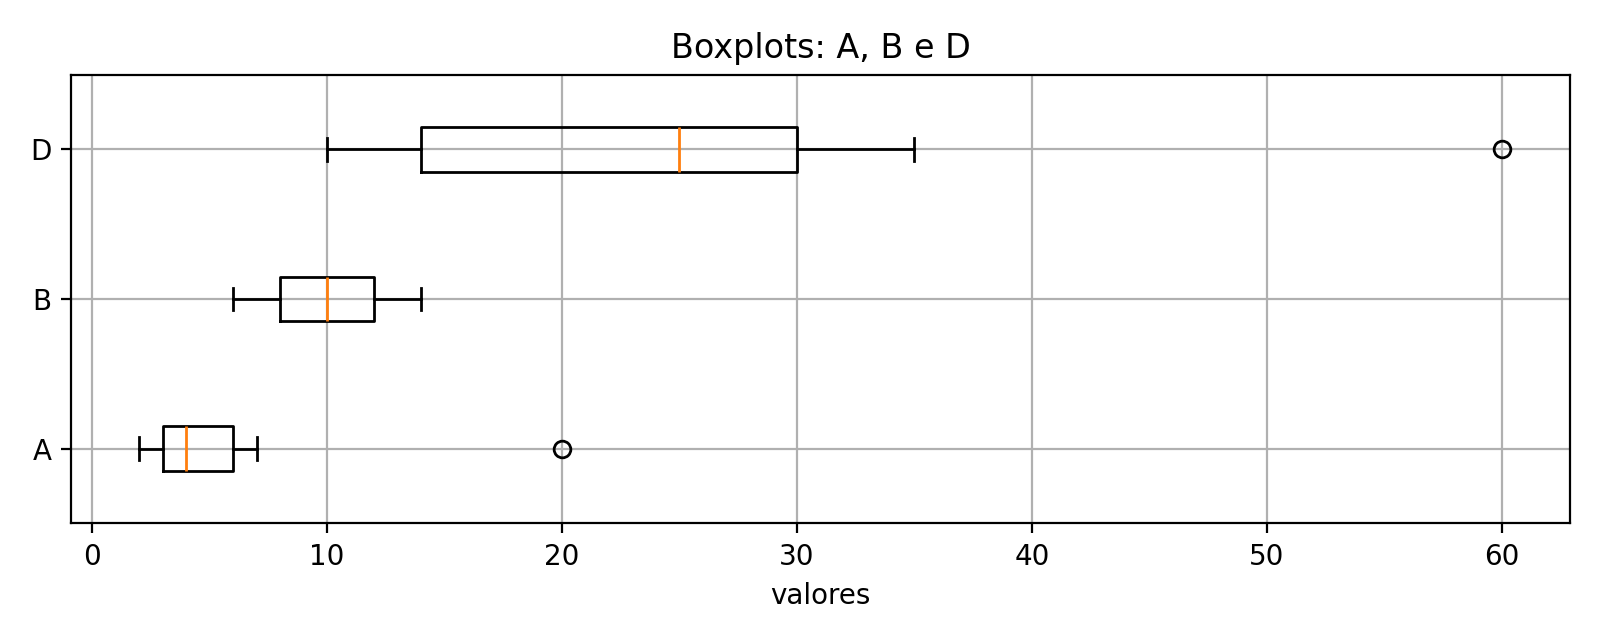
\includegraphics[width=0.9\linewidth]{figs/boxplot_bowley.pdf}
\caption{Boxplots: $A$, $B$ e $D$ (exemplo do Bowley).}
\label{fig:boxplot_bowley}
\end{figure}

\begin{example}
    
Se $p_0=\text{R\$ }50$ e $p_t=\text{R\$ }65$, então:
\[
p_{0,t}=\frac{65}{50}=1{,}30,
\]
ou seja, houve aumento de \(30\%\) em relação à base.

\end{example}

%==================================================
\subsection{Índices Agregativos Ponderados}

Para um conjunto de bens, utilizam-se pesos baseados na participação de cada bem no valor total.

\subsubsection*{Laspeyres ($L$)}

Utiliza ponderação da época base:
\[
LP_{0,t}=\frac{\sum p_{it}q_{i0}}{\sum p_{i0}q_{i0}},
\qquad
LQ_{0,t}=\frac{\sum p_{i0}q_{it}}{\sum p_{i0}q_{i0}}.
\]

\subsubsection*{Paasche ($P$)}

Utiliza ponderação da época atual:
\[
PP_{0,t}=\frac{\sum p_{it}q_{it}}{\sum p_{i0}q_{it}},
\qquad
PQ_{0,t}=\frac{\sum p_{it}q_{it}}{\sum p_{it}q_{i0}}.
\]

\subsubsection*{Fisher ($F$)}

É a média geométrica entre Laspeyres e Paasche:
\[
FP_{0,t}=\sqrt{LP_{0,t}\,PP_{0,t}}.
\]

\subsubsection*{Marshall-Edgeworth ($M$)}

Utiliza como peso a soma das quantidades das duas épocas:
\[
MP_{0,t}=\frac{\sum (q_{i0}+q_{it})\,p_{it}}{\sum (q_{i0}+q_{it})\,p_{i0}}.
\]

\subsubsection*{Divisia (média geométrica ponderada)}

\[
DP_{0,t}=\prod_{i=1}^{n}\left(\frac{p_{it}}{p_{i0}}\right)^{w_{i0}}.
\]

\begin{example}
    Se \(LP=1{,}2353\) e \(PP=1{,}2365\), então:
\[
FP=\sqrt{1{,}2353\times 1{,}2365}\approx 1{,}2359.
\]
\end{example}

\subsection{Aplicação: Deflacionamento}

Esses instrumentos permitem realizar o \textbf{deflacionamento}, isto é, usar um índice de preços para eliminar o efeito da inflação e determinar o valor real em uma data-base.

\subsubsection*{Cálculo do Valor Real}

Se o índice estiver em forma decimal (por exemplo, \(I=1,0527\)):
\[
V_{\text{real}}=\frac{V_{\text{nominal}}}{I}.
\]
Se o índice estiver em base 100, multiplica-se por 100:
\[
V_{\text{real}}=\frac{V_{\text{nominal}}}{I}\times 100.
\]

\subsubsection*{Poder Aquisitivo}

\[
PA=\frac{1}{I}.
\]

\begin{example}
    Salário nominal: \(\text{R\$ }2.500,00\). \quad Índice: \(I=1{,}0527\).
    \[
    V_{\text{real}}=\frac{2500}{1,0527}\approx 2374,85.
    \]
\end{example}



